\documentclass[ignorenonframetext]{beamer}
\usepackage[utf8]{inputenc}
\usepackage[T1]{fontenc}
\usepackage[english]{babel}
\usepackage{tikz}
\usepackage{pifont}
\usepackage{pgf}
\usepackage{pgfplots}
\usepackage{listings}
%\usepackage[round]{natbib}
\usetikzlibrary{arrows,  automata}
\lstset{}
\usetikzlibrary{shapes.geometric}
\usetikzlibrary{positioning}
\usetikzlibrary{shapes.geometric}
\usepackage{graphicx}
\usepackage{sansmathaccent}
\usepackage{hyperref}
\usepackage{bibentry}
\usepackage{color, soul}
\usepackage{epstopdf}
\usepackage[absolute,overlay]{textpos}
\usepackage{graphicx}

\usetheme{Luebeck}
\useinnertheme{default} % circles, rounded, rectangles
\usefonttheme{structurebold}
\setbeamertemplate{navigation symbols}{} % hide navigation symbols

\setbeamertemplate{sections/subsections in toc}[sections numbered]
\usetikzlibrary{shapes.geometric}
\title[Seminar Presentation]{Prioritized Sweeping Neural DynaQ: Neural Networks over All?}
\author{Alexander Andreevi\v{c} Osiik}
\institute{Universität zu Lübeck}
\date{January 17th 2020}
\setbeamertemplate{headline}{}

    \expandafter\def\expandafter\insertshorttitle\expandafter{%
	\insertshorttitle\hfill%
	\insertframenumber\,/\,\inserttotalframenumber}
\begin{document}
	\frame<presentation>{\titlepage}
		\mode<article>{\maketitle
		\tableofcontents}
	
%% EINLEITUNG
	\section*{Introduction}
\begin{frame}
\frametitle{Introduction}
\begin{itemize}
	\item In recent years, \textbf{reinforcement learning} has gained a lot of popularity due to some spectacular successes
	\end{itemize}
\begin{tikzpicture}
\uncover<2->{\node (img1)[xshift = -3cm, yshift = -1cm] {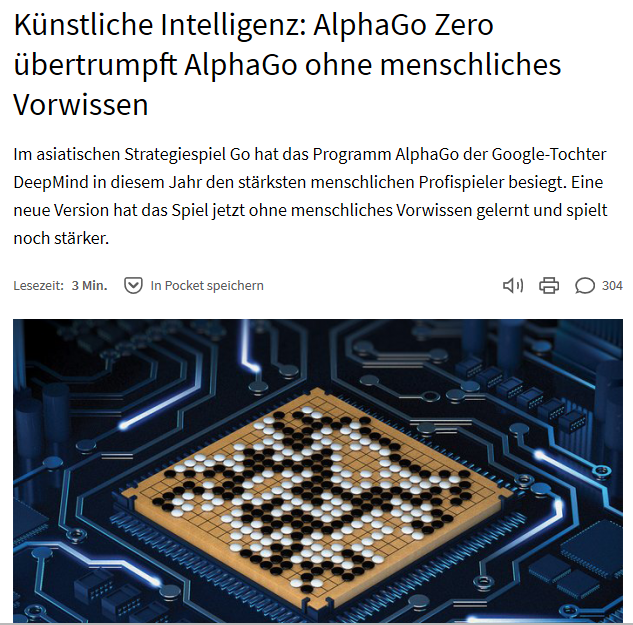
\includegraphics[height=5cm]{Images/AlphaGo}};}

\uncover<3->{\node (img2) {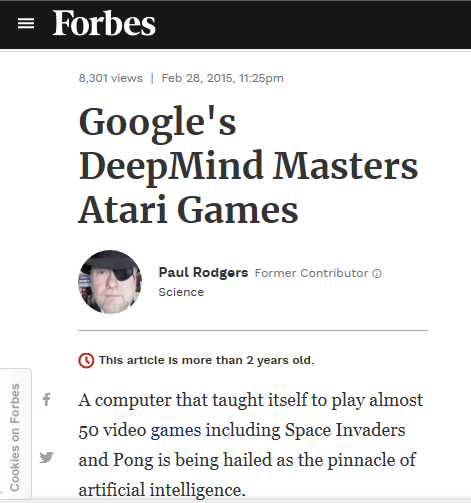
\includegraphics[height=5cm]{Images/DeepMind}};}
\pause
\uncover<4->{\node (img3) at (img1)
	{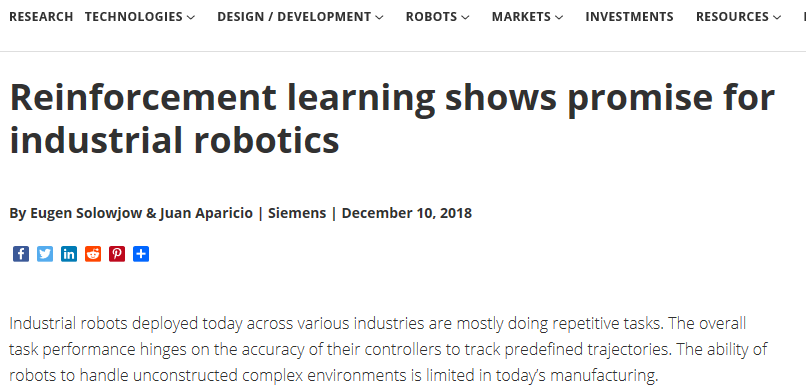
\includegraphics[height=4cm]{Images/Robotics}};}
\end{tikzpicture}
\end{frame}

\begin{frame}
\frametitle{Introduction}
\begin{itemize}
	\item \textbf{Reinforcement learning} (RL) is based on learning processes of biological systems
	\uncover<2->{\item \textbf{Supervised learning}: create a model based on training set to classify input}
	\uncover<3->{\item \textbf{Unsupervised learning}: sort data structures through cluster analysis}
\end{itemize}
\begin{figure}
	\begin{center}
		\vspace*{-.7cm}
		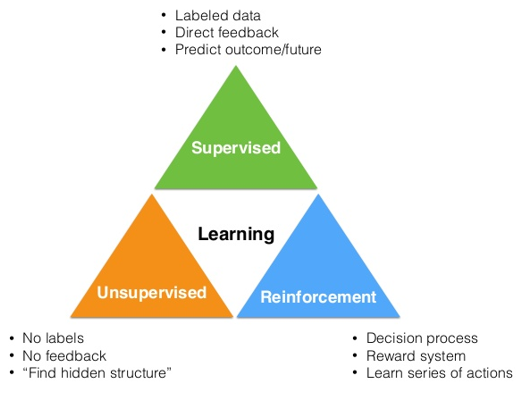
\includegraphics[height=4.5cm]{Images/LearningPyramid}
		\caption{Categories of Machine Learning \cite{Dishpande}}
	\end{center}
\end{figure}
\end{frame}

\begin{frame}
	\frametitle{Limitations}
	Although RL can be effectively applied to some problems, there are some limitations:
	\vspace*{.6cm}
	\begin{itemize}
 		\uncover<2->{\item Parameters affect speed of learning}
		\uncover<3->{\item Reward function is required}
		\uncover<4->{\item Storage of world models: computing-heavy and time-consuming for large dynamic environments}
		\uncover<5->{\item  RL is still orders of magnitude above a practical level of sample efficiency \cite{BlogRL}}
		\uncover<6->{\item[$\implies$] The last two problems are tackled by Aubin et. al \cite{NeuralDynaQ}}
	\end{itemize}
\end{frame}

\begin{frame}
\frametitle{Paper topic}
	Recent progress in reinforcement learning: Development of GALMO for Prioritized Sweeping Neural DynaQ Learning by \cite{NeuralDynaQ}.\\
	\vspace{1cm}
	This solution promises to boost learning due to offline replays, a model of the \textit{hippocampal replays} that occur in rodents.\\
	\vspace{1cm}
	GALMO architecture can also associate multiple outputs to a single input.
\end{frame}

\begin{frame}
\frametitle{Outline}
\begin{enumerate}\large{
\item Introduction \checkmark\vspace*{.4cm}
\item \textbf{Biological background}\vspace*{.4cm}
\item RL Definitions\vspace*{.4cm}
\item GALMO\vspace*{.4cm}
\item Project and Results}
\end{enumerate}
\end{frame}

\section*{Biological background}
\begin{frame}
\frametitle{Biological background}
The hippocampus is the main memory of the brain and the switch point between short-term and long-term memory.
\begin{itemize}
	\uncover<2->{\item Disturbance in this area leads to loss of the ability to store new information \cite{OKEEFE1971171}, \cite{Maguire}
	\item[$\implies$] Learning no longer possible!}
\end{itemize}
\begin{center}
	\hspace*{4cm}
	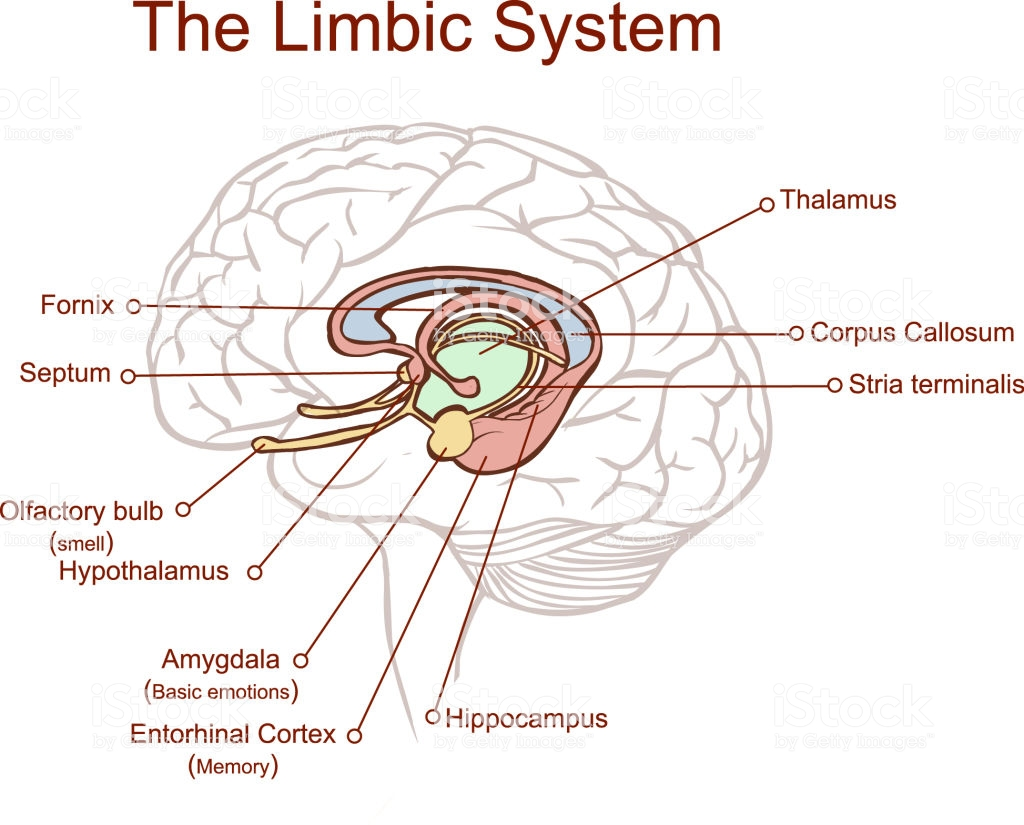
\includegraphics[height=5cm]{Images/hypo2}
\end{center}
\end{frame}

\begin{frame}
\frametitle{Biological background}
\cite{OKEEFE1971171} discovered the presence of \textit{place cells} in the hippocampus.\\
\begin{itemize}
	\uncover<2->{\item Interaction with the environment leads to activation of these cells}
	\uncover<2->{\item[$\implies$] Postulation, that the hippocampus functions as a spatial map}
	\uncover<3->{\item It has also been observed that activations occur during rest or sleep, at significally faster pace}
\end{itemize}
\begin{center}
	\uncover<2->{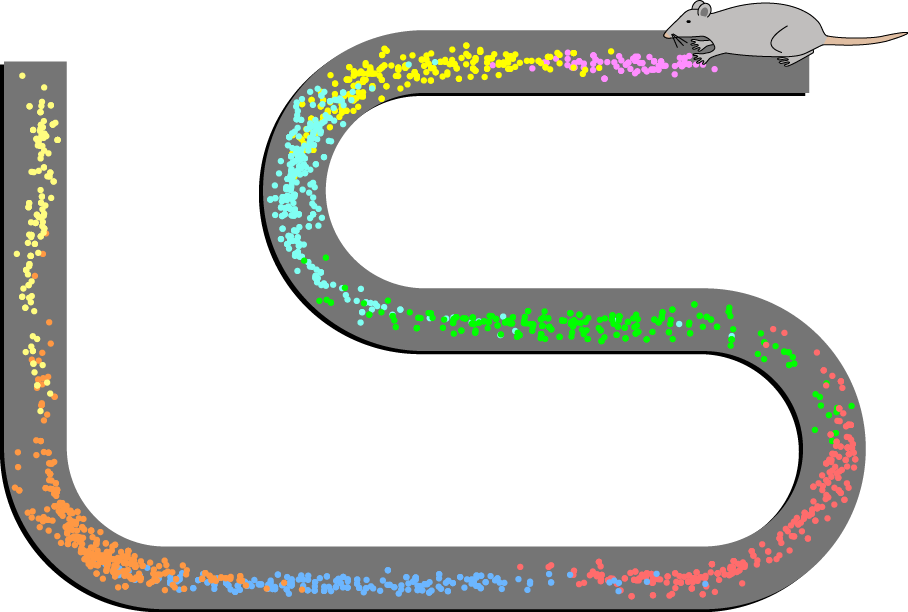
\includegraphics[height = 2cm]{Images/Place_Cell_Spiking_Activity_Example}}
	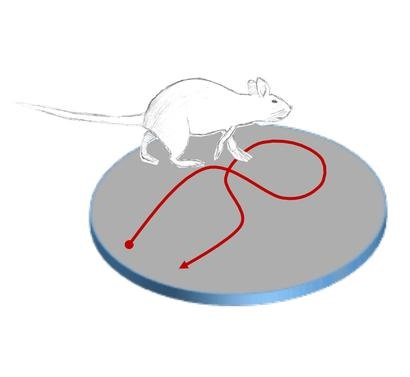
\includegraphics[height=3cm]{Images/Replay1}
	\uncover<3->{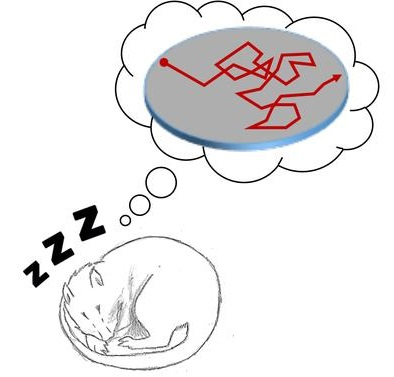
\includegraphics[height=3cm]{Images/Replay2}}
\end{center}
\uncover<4>{\begin{block}{Goal: Convert reactivation of place cells into a RL model}
\end{block}}
\end{frame}

\begin{frame}
\frametitle{Outline}
\begin{enumerate}\large{
		\item Introduction \checkmark\vspace*{.4cm}
		\item Biological background \checkmark\vspace*{.4cm}
		\item \textbf{RL Definitions}\vspace*{.4cm}
		\item GALMO\vspace*{.4cm}
		\item Project and Results}
\end{enumerate}
\end{frame}

\section*{Modeling of Reinforcement Learning}
\begin{frame}
\frametitle{Markov Decision Process}
MDP is a framework for modeling an agent’s decision making in an environment
\vspace*{.5cm}
\begin{itemize}
\uncover<2->{\item Set of states $S:$ $\{s_1,s_2,\dots, s_n\}$}\vspace{0.3cm}
\uncover<2->{\item Set of actions $A:$  $\{a_1,a_2,\dots, a_n\}$ }\vspace{0.3cm}
\uncover<2->{\item Transition function $T: S\times A \times S$, which is the probability of going from state $s$ to state $s'$ via action $a$}\vspace{0.3cm}
\uncover<3->{\item  Reward function $R: S\times A \times S \rightarrow \mathbb{R}$}\vspace{0.3cm}
\uncover<4->{\item[$\implies$] Goal is to find policy $\Pi$, where an optimal action is assigned to each state}
\end{itemize}
\end{frame}

\begin{frame}
	\frametitle{V-values and Q-values}
	MDP contains a \textit{value function} $V$ for its \textit{states}. It is the expected reward for being in a state $s \in S$
	$$V^*(s) = \max_{a \in A} \sum_{s' \in S}^{} T(s,a,s')[R(s,a,s')+\gamma V^*(s')]$$
	$\gamma\in [0,1]$: Exploration factor
%	\begin{textblock*}{5cm}(3cm,1cm) % {block width} (coords)
%		
\includegraphics[height= 2cm]{Images/ExplorationExploitation}
%	\end{textblock*}
	\begin{textblock*}{5cm}(8cm,3.5cm) % {block width} (coords)
	\uncover<2->{
\includegraphics[height= 1.8cm]{Images/ExplorationExploitation}}\end{textblock*} \vspace{1cm}
	\uncover<3->{What if there is no model of the environment (= no knowledge about states)?}\\
	\uncover<4->{$\implies$ Use the \textit{action value function} $Q$ instead 
	$$Q^*(s,a) = \max_{a \in A} \sum_{s' \in S}^{} T(s,a,s')[R(s,a,s')+\gamma \max_{a' \in A}Q^*(s',a')]$$}
\end{frame}
\begin{frame}
	\frametitle{Q-learning}
	The function $Q(s,a)$ can be estimated using \textbf{Q-Learning}.
	The value $Q(s,a)$ is iteratively updated using the Bellman Equation:
	$$Q(s,a) \leftarrow Q(s,a) + \alpha [r + \gamma \max_{a' \in A}Q(s',a')-Q(s,a)]$$$$\alpha: \text{Learning rate}$$
	The values are stored  in a \textbf{Q-table}, where each cell $(s\in S, a \in A)$ represents the highest achievable reward performing action $a$ in state $s$.\\
\end{frame}
\begin{frame}
	\frametitle{Q-learning}
	The amount of time to explore and store each state in the Q-table would be incredibly large for large environments.\\ \vspace*{1cm}  
	In \textbf{Deep Q-learning} (DQN), neural networks are used to approximate the Q-value function, where the state is the network's input and the Q-values of all actions are its output.
	\begin{figure}
		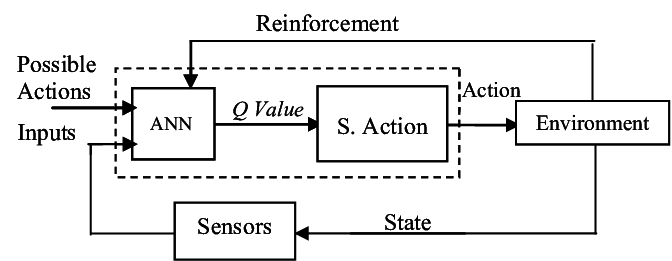
\includegraphics[height = 3cm]{Images/RL_ANN}
		\cite{HatemRL}
	\end{figure}
	
\end{frame}

\begin{frame}
\frametitle{Outline}
\begin{enumerate}\large{
		\item Introduction \checkmark\vspace*{.4cm}
		\item Biological background \checkmark\vspace*{.4cm}
		\item RL Definitions \checkmark\vspace*{.4cm}
		\item \textbf{GALMO}\vspace*{.4cm}
		\item Project and Results}
\end{enumerate}
\end{frame}

\section*{GALMO}
\begin{frame}
	\frametitle{Experimental setup}
	\cite{NeuralDynaQ} set up an experimental task environment.\\
	\begin{itemize}
		\item Two successive T-mazes with return corridors
		\item Decision points T1 and T2
		\item Rewarding food pellets at each side\\
		\begin{center}
			\begin{tikzpicture}
			\node (img1) {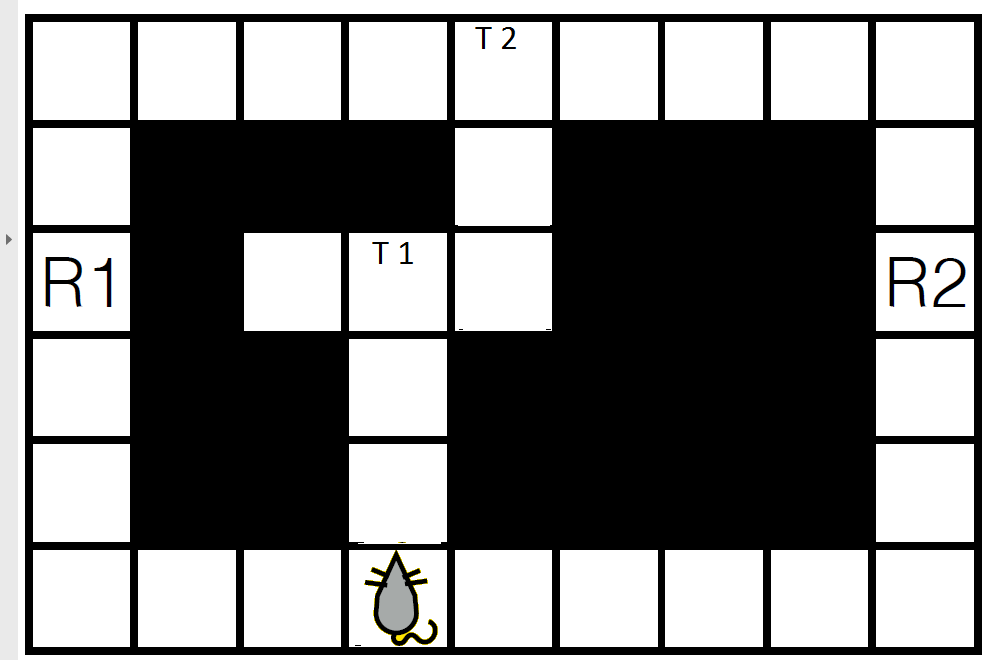
\includegraphics[height = 3cm]{Images/Setup0}};
			\uncover<2>{\node (img2) at (img1) {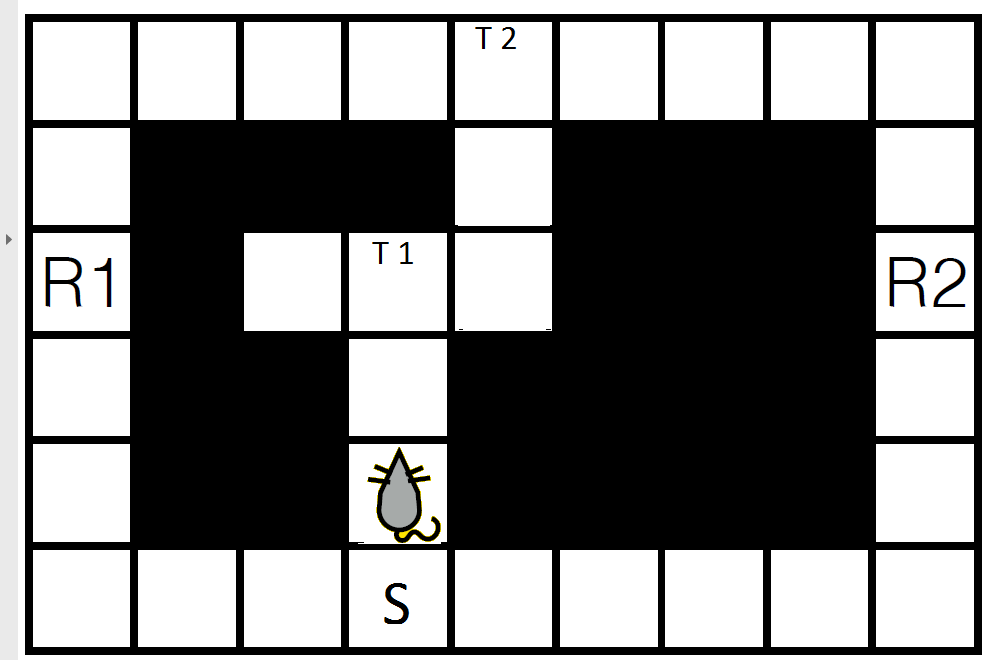
\includegraphics[height = 3cm]{Images/Setup1}};}
			\uncover<3>{\node (img4) at (img1) {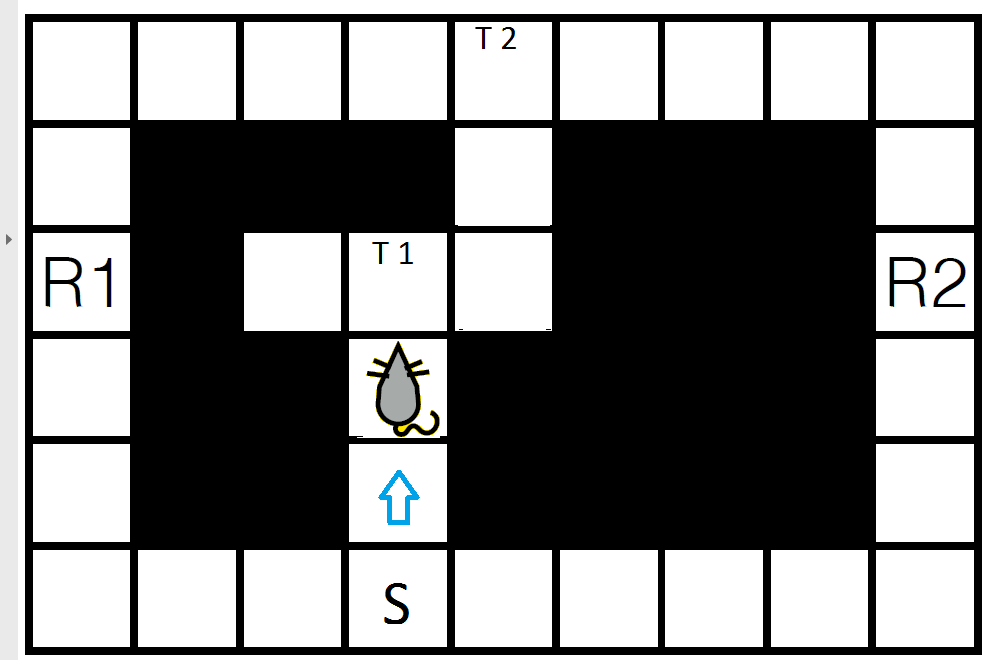
\includegraphics[height = 3cm]{Images/Setup2}};}
			\uncover<4>{\node (img3) at (img1) {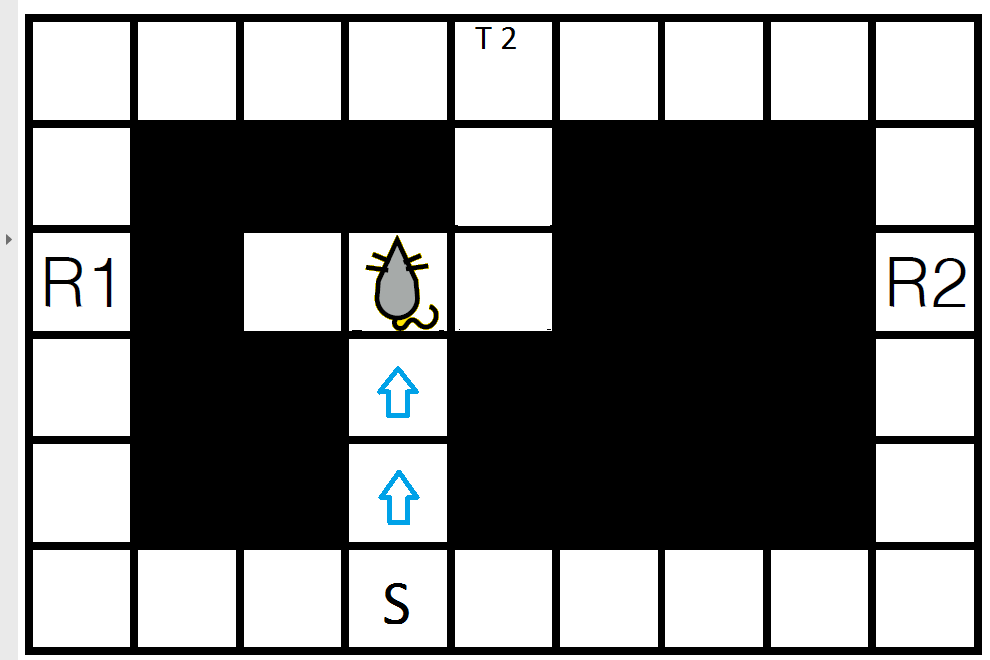
\includegraphics[height = 3cm]{Images/Setup3}};}
			\uncover<5>{\node (img3) at (img1) {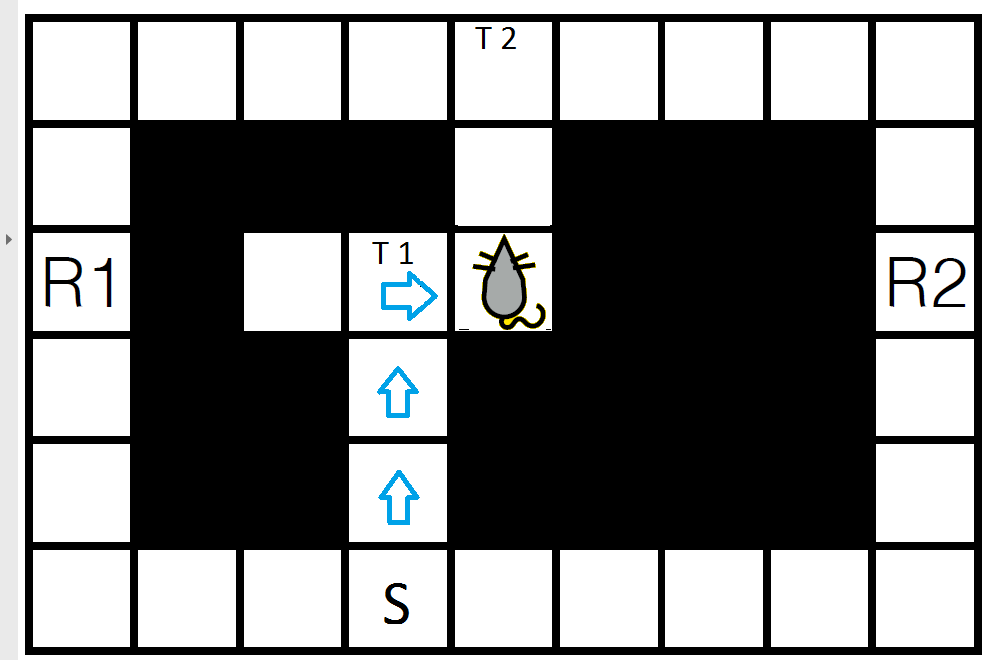
\includegraphics[height = 3cm]{Images/Setup4}};}
			\uncover<6>{\node (img3) at (img1) {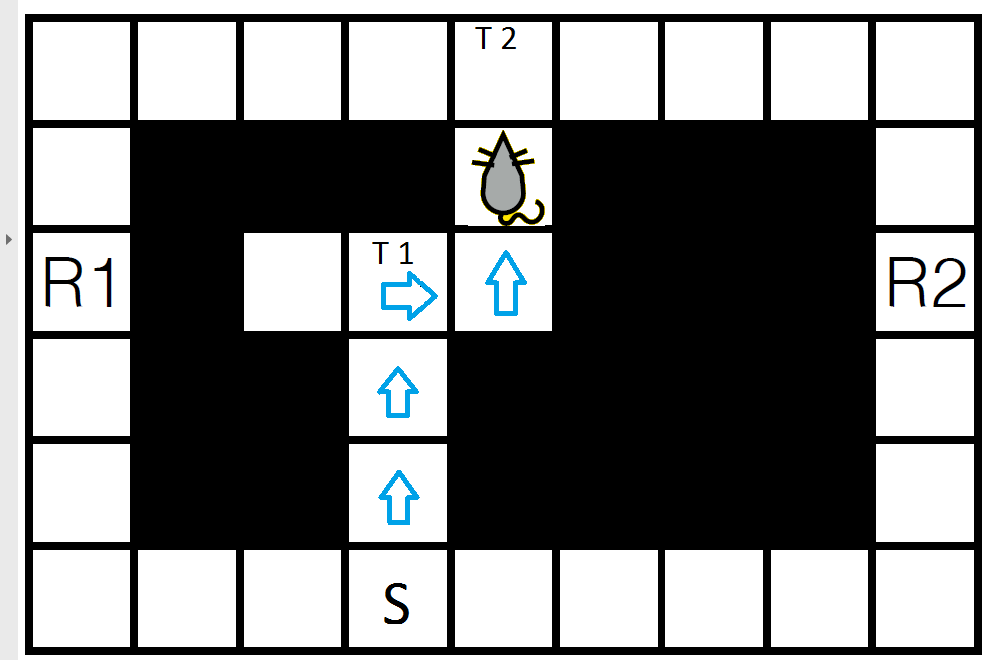
\includegraphics[height = 3cm]{Images/Setup5}};}
			\uncover<7>{\node (img3) at (img1) {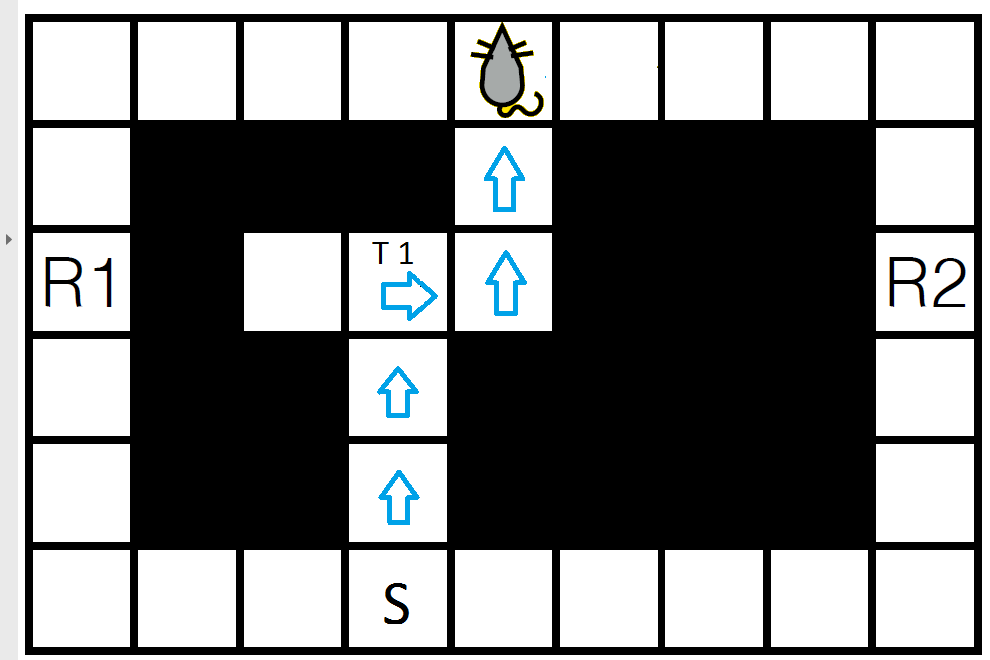
\includegraphics[height = 3cm]{Images/Setup6}};}
			\uncover<8->{\node (img3) at (img1) {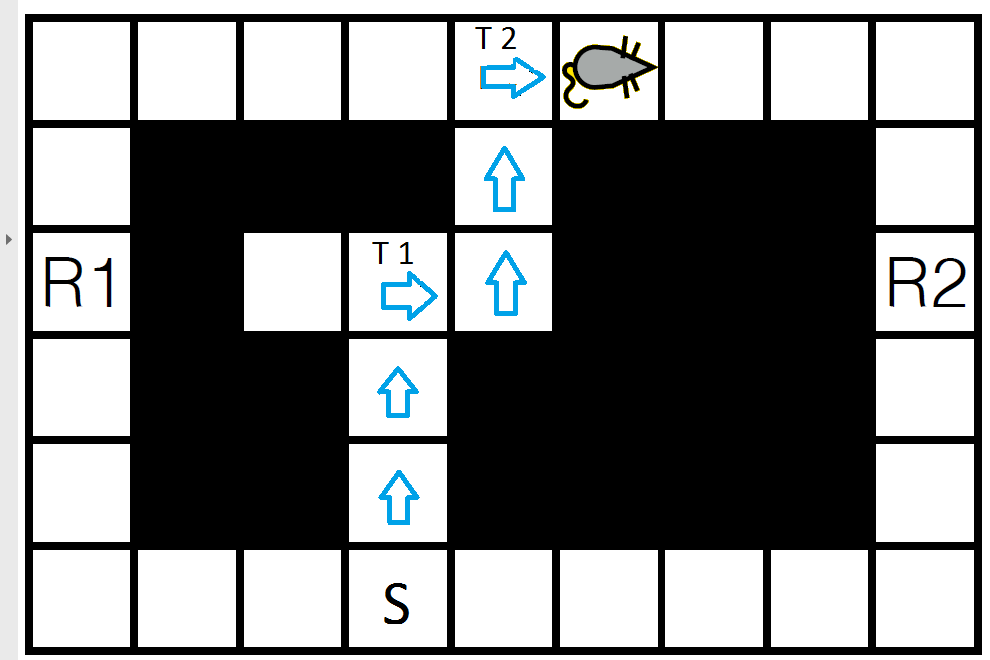
\includegraphics[height = 3cm]{Images/Setup}};}
			\end{tikzpicture}
		\end{center}
		\uncover<9>{\item Three tasks were given:\begin{enumerate}
			\item go to left side
			\item go to right side
			\item alternate between left and right}
		\end{enumerate}
	\end{itemize}
\end{frame}

\begin{frame}
	\frametitle{Experimental setup}
	The agent's state is a concatenation of 32 location components and 2 reward memory components (left and right).\\\vspace*{0.3cm}
	A problem was encountered, namely that some states may have more than one predecessor.\\
	\begin{figure}
		\begin{center}
			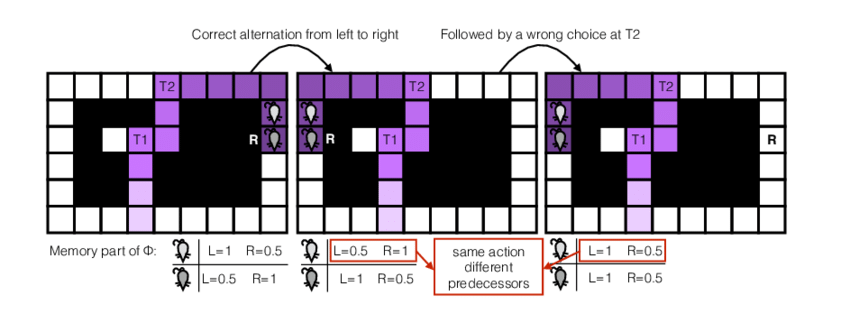
\includegraphics[height=3.5cm]{Images/MultiplePredecessors}
			\caption{Multiple predecessors for same location\cite{NeuralDynaQ}}
		\end{center}
	\end{figure}
\end{frame}

\begin{frame}
	\frametitle{GALMO}
	To confront this issue, a \textit{growing algorithm to learn multiple outputs} (GALMO) was created.
	\begin{itemize}
		\item Algortihm creates multiple neural neworks $N_i$ coupled with a gating network (\textit{mixture of expert} \cite{AdaptiveMixture})
		\item Creates a new network on the fly when outlier is detected (Assumption: outlier is caused by an input that should predict multiple outputs). Specializes each network to a predecessor
		\begin{center}
			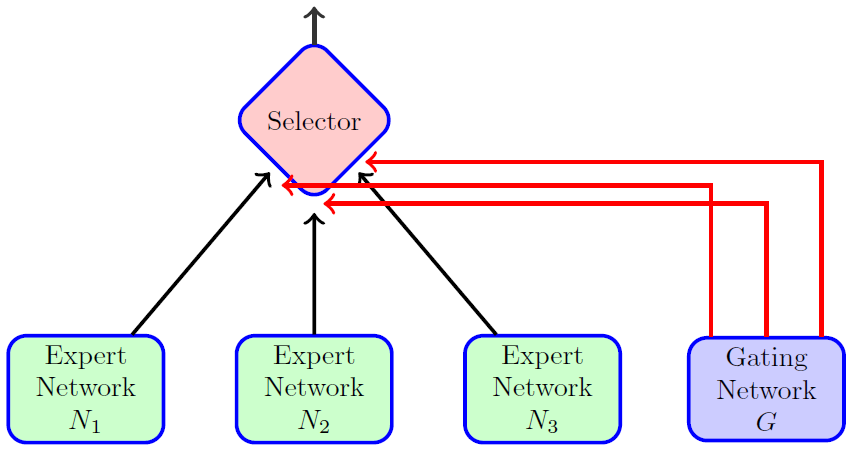
\includegraphics[height = 3cm]{Images/Gating}
		\end{center}
	\end{itemize}
\end{frame}
\begin{frame}
	\frametitle{Dyna-Q}
	Second part of the algorithm was neural \textit{Dyna-Q} with \textit{prioritized sweeping}.\\
	\textit{Dyna} is an architecture that mixes direct RL updates and planning updates:
	\begin{itemize}
		\item Agent creates a model from environment experience during initial exploration
		\item Policy is updated using simulated experience from the model and actual experience \\
		\uncover<2>{$\implies$ Simulated experience replays are treated as model for hippocampal replays! }
	\end{itemize} 
\end{frame}

\begin{frame}
\frametitle{Outline}
\begin{enumerate}\large{
		\item Introduction \checkmark\vspace*{.4cm}
		\item Biological background \checkmark\vspace*{.4cm}
		\item RL Definitions \checkmark\vspace*{.4cm}
		\item GALMO \checkmark\vspace*{.4cm}
		\item Project and Results}
\end{enumerate}
\end{frame}

\begin{frame}
\frametitle{GALMO Results}
A framework to analyze the role of hippocampal replays in the learning process was desired. \\
\vspace*{0.5cm}
The state activation analysis has shown that around 15-20\% of state reactivations during replays correspoded to actual 3-step sequences. 
\\Unfortunately, no clear pattern could be found comparing the state reactivations during the three tasks. 
\end{frame}
\begin{frame}
	\frametitle{GALMO Results}
	The network architecture proposed by \cite{NeuralDynaQ} was able to learn multiple predecessor cases. Overall, the system solved all tasks faster than the corresponding Q-learning system. 
	\begin{figure}
		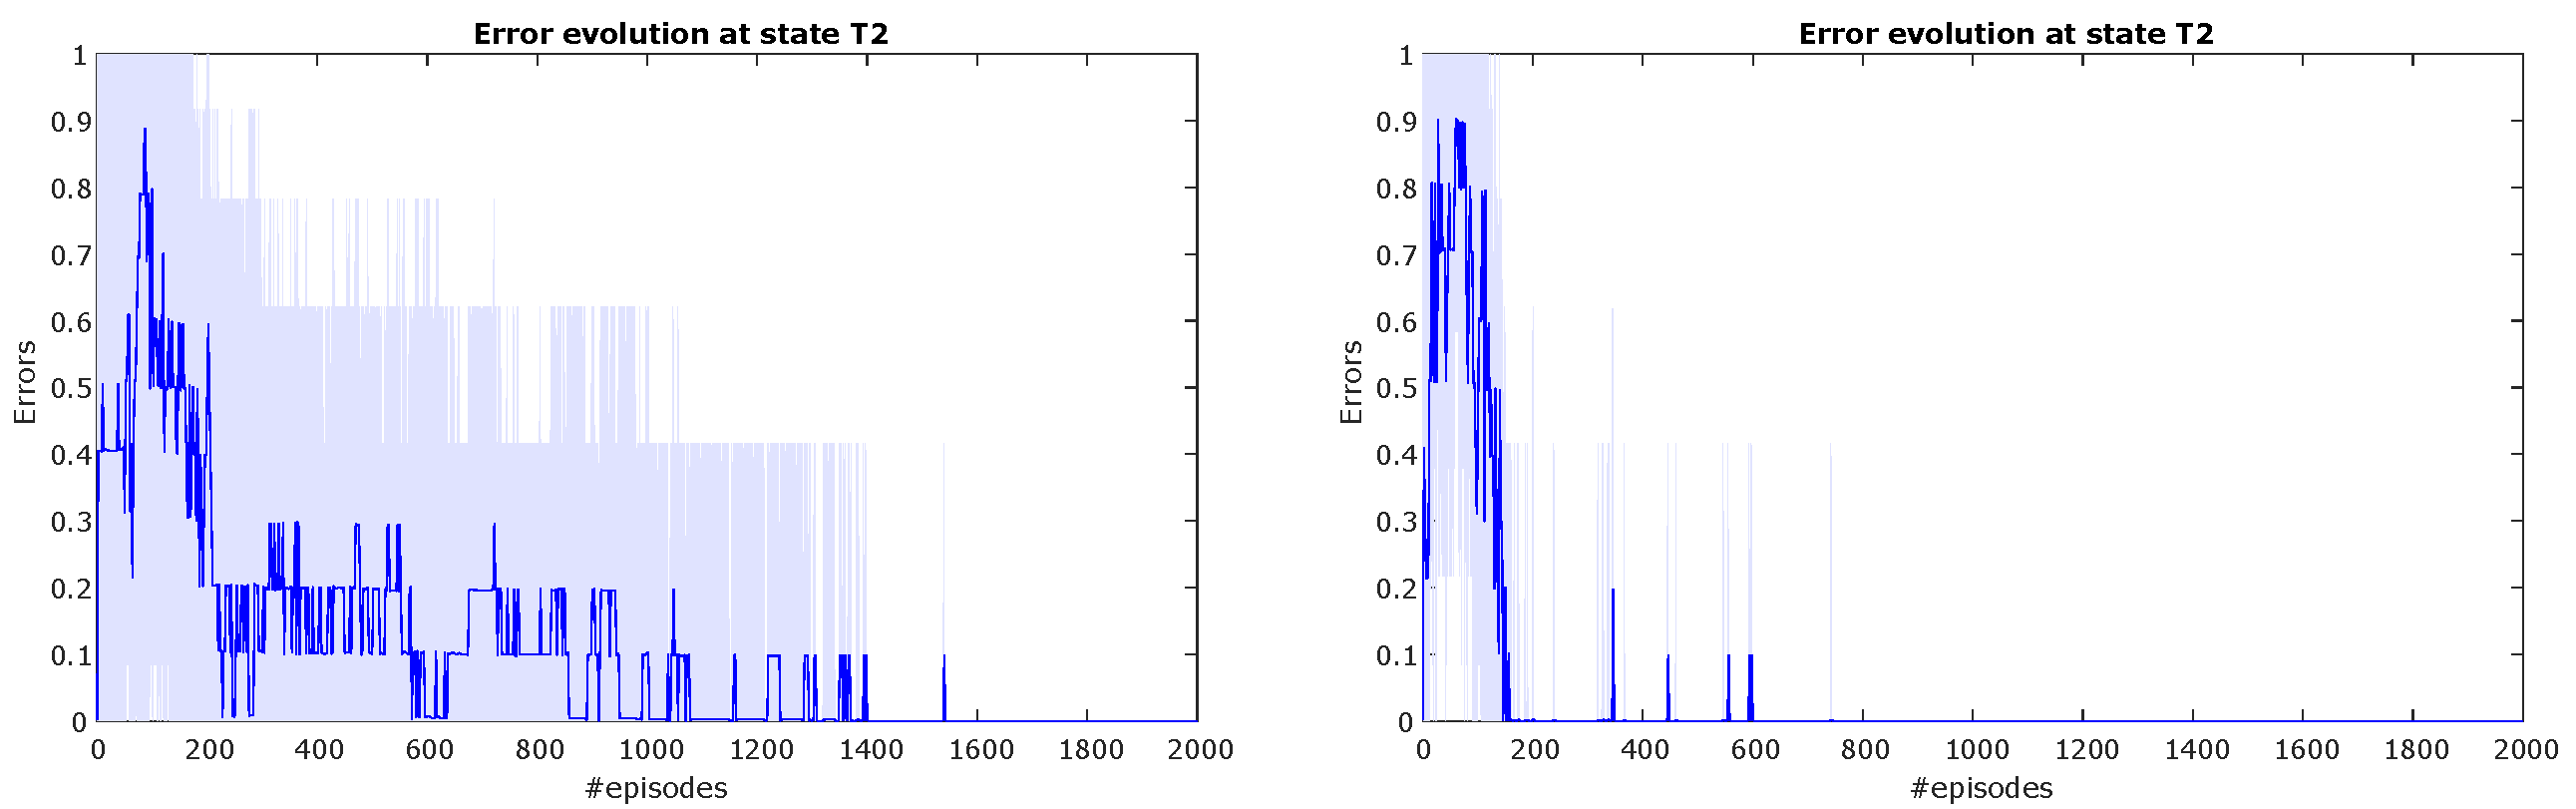
\includegraphics[height=3cm]{figs/QvsDyna2}
		\caption{Learning without and with replays \cite{NeuralDynaQ}}
	\end{figure}
	Unfortunately, no information was given on the duration of the networks' learning, which would be interesting concerning a cost-benefit calculation.
\end{frame}
\begin{frame}
	\frametitle{Project}
	As a practical part, the experimental environment and Q-learning were implemented in Python. The goal was 
	\begin{itemize}
		\item to enhance the understanding of structures and procedures in Reinforcement Learning
		\item to create comparative results of a Q-learning implementation 
	\end{itemize}
\begin{center}
	\begin{tikzpicture}
	\uncover<2->{\node (img1)[xshift = -2cm] {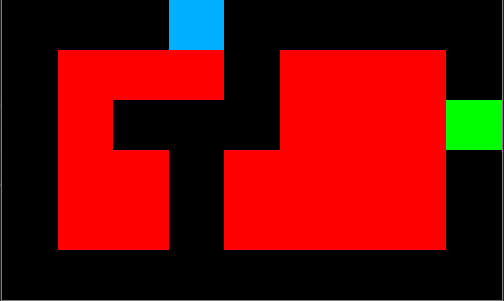
\includegraphics[height=3cm]{Images/Environment}};}
	
	\uncover<3->{\node (img2) {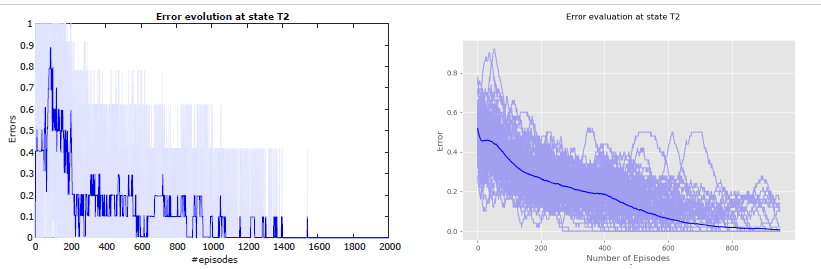
\includegraphics[height=3.1cm]{Images/comp}};}
	\pause
	\end{tikzpicture}
\end{center}
\uncover<3>{The own results were slightly better than the corresponding Q-learning due to initial modification, but ultimately can not surpass the Neural Dyna-Q with prioritized sweeping.}
\end{frame}


%% DANKSAGUNG
\begin{frame}
\begin{center}
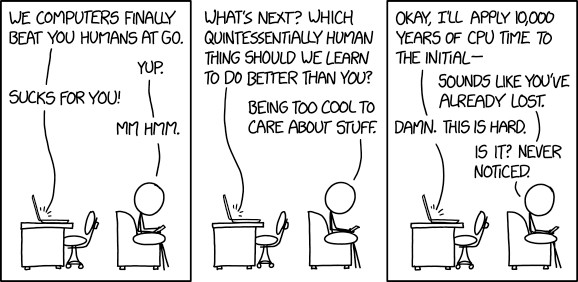
\includegraphics[height=3cm]{Images/XKCD}\\ \vspace*{.5cm}
Thank you for your attention!

\end{center}
\end{frame}

%%BIBLIOGRAPHY
\begin{frame}
	\bibliographystyle{apalike}
	\bibliography{main}
\end{frame}

\end{document}